

\chapter{Algorithmen zur Pfadplanung}
\section{Definition von Pfadplanungsalgorithmen}
 

Algorithmen zur Pfadplanung sind schwierig mathematisch präzise zu definieren.
In \cite[~S. 19]{Lav06} wird der Begriff Algorithmus definiert und anschließend so erweitert, dass er den Ansprüchen der Pfadplanungsaufgabe entspricht. 
Eine \textit{Turing Maschine}\index{Turing Maschine} repräsentiert einen Algorithmus und ist nach der \textit{Church-Turing These}\index{Church-Turing These}, \textit{Turing vollständig} und damit berechenbar \cite{Schmitz:19}. 
Der Definition fehlt die Repräsentation der Interaktion eines Roboters mit der Umgebung, wie sie in Abbildung \ref{lav01} dargestellt wird. 
Daher wird ein Planer\index{Planer} als ein Algorithmus definiert, welcher einen Plan\index{Plan} konstruiert. 
Der Planer kann einer Turing Maschine entsprechen. 
Er kann damit sowohl eine Maschine, als auch ein Mensch\footnote{intuitiv berechenbar bedeutet in der Church-Turing These, auch vom Mensch berechenbar.} sein.
Er ist aber nicht darauf limitiert, sondern kann den Ansprüchen entsprechend erweitert werden.\cite[~S. 20]{Lav06}

\begin{figure} % Hier lieber eine eigene Kombination an Grafiken
	\centering
	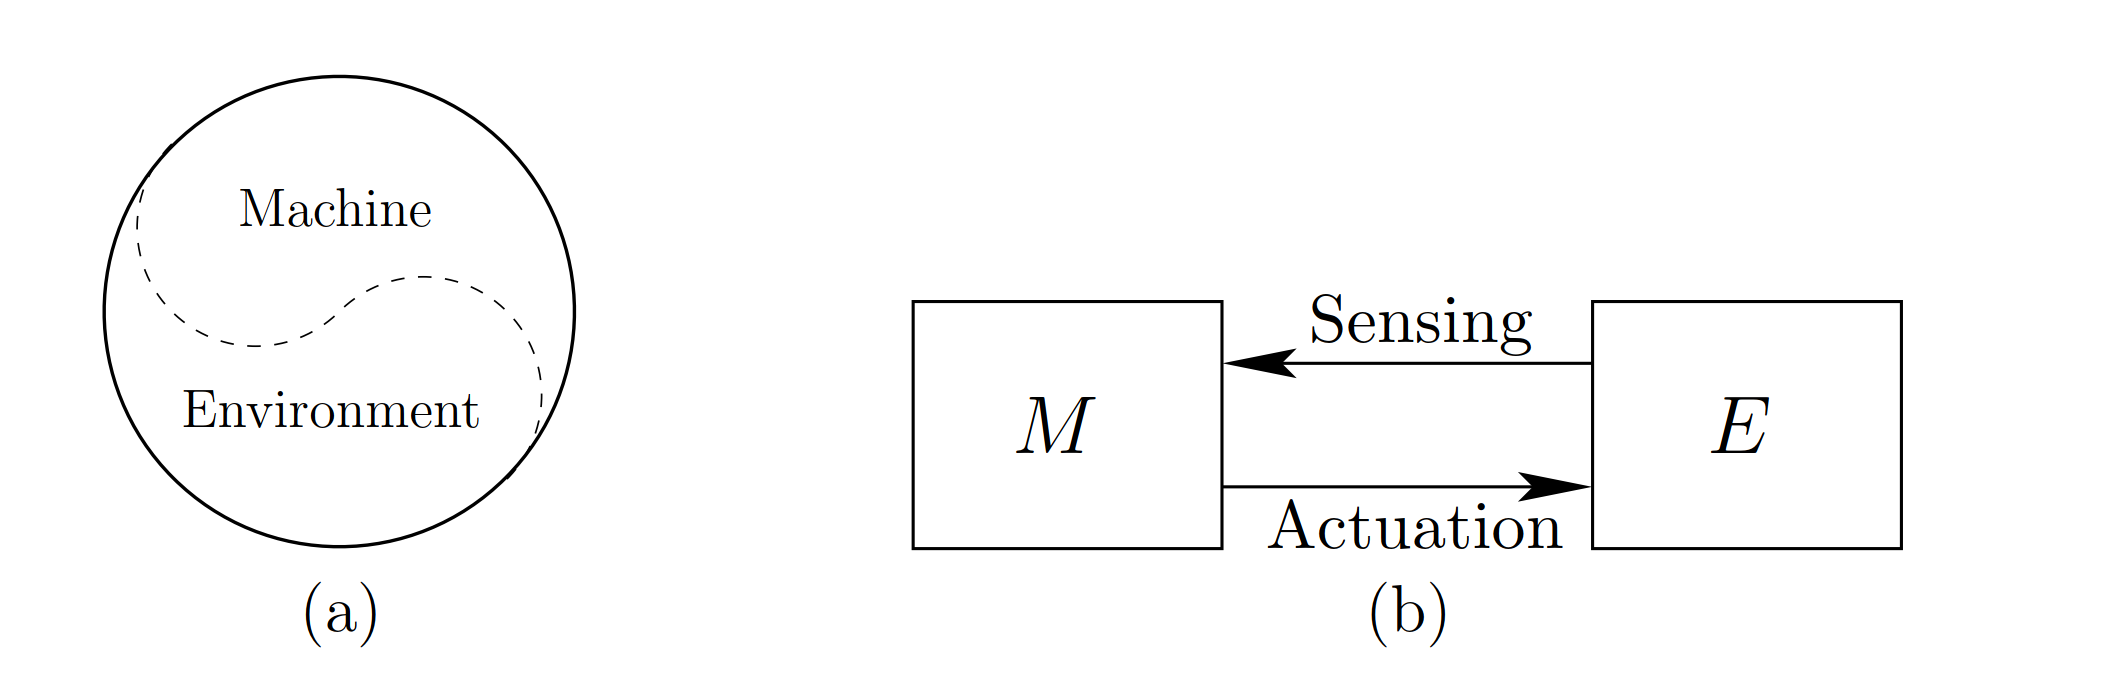
\includegraphics[width=0.75\textwidth]{images/img224.png}
	\caption{Abb. 1.5 von \cite[~S. 20]{Lav06}:  (a) Die Grenze zwischen Maschine und Umgebung ist fließend, es ist eine Linie die stark in Abhängigkeit vom Kontext gezogen wird. (b) Ist die Grenze festgelegt, wird angenommen, dass die Maschine $M$ mit der Umgebung $U$ durch Sensorik und den Antrieb interagiert.}
	\label{lav01}
\end{figure}

Ein Plan, kann drei unterschiedliche Funktionen erfüllen.
%Ausführung
Für die \textit{Ausführung}\index{Ausführung} der Anweisungen durch einen Roboter, kann im ersten Fall eine kodierte Eingabe für eine Maschine erstellt werden. 
Diese kann dadurch programmiert werden, wird damit bei der Ausführung autonom und kann nicht mehr mit dem Planer interagieren.
Im zweiten Fall erzeugt der Planer eine Spezialmaschine, welche dazu entworfen ist die Aufgabe zu lösen.\cite[~S. 21]{Lav06}\newline\\
%Verbesserung 
Eine \textit{Verbesserung}\index{Verbesserung} der Eigenschaften, in bestimmten Parametern kann erreicht werden, indem der Plan als Eingabe einem Planer übergeben wird. Anhand von Abbildung \ref{lav02} wird ersichtlich, wie der gleiche Plan verbessert werden kann, indem verschiedene Aspekte der Problemstellung fokussiert werden.\cite[~S. 22]{Lav06}

\begin{figure}
	\centering
	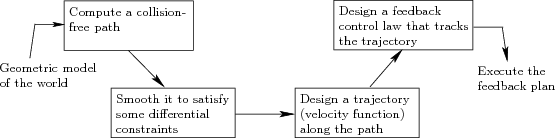
\includegraphics[width=0.75\textwidth]{images/img247.png}
	\caption{Abb. 1.5 von \cite[~S. 20]{Lav06}:  Ein Verbesserungsprozess, der sich in der Robotik bewährt hat.}
	\label{lav02}
\end{figure}

Bei der \textit{Hierarchischen Inklusion}\index{hierarchische Inklusion} werden Pläne als Aktionen, in einen größeren Plan aufgenommen. In Abbildung \ref{cortes01} sieht man einen Roboter der ein Objekt mehrmals hintereinander manipulieren muss, bevor er es aufnehmen kann, um an das Ziel zu kommen \cite{cortes:03}. Dazu wird das Planungsproblem in mehrere Unterprobleme zerteilt. Es entsteht eine hierarchische Baumstruktur, in der ein Hauptplan aus mehreren Plänen besteht\cite[~S. 23]{Lav06}.

\begin{figure}
	\centering
	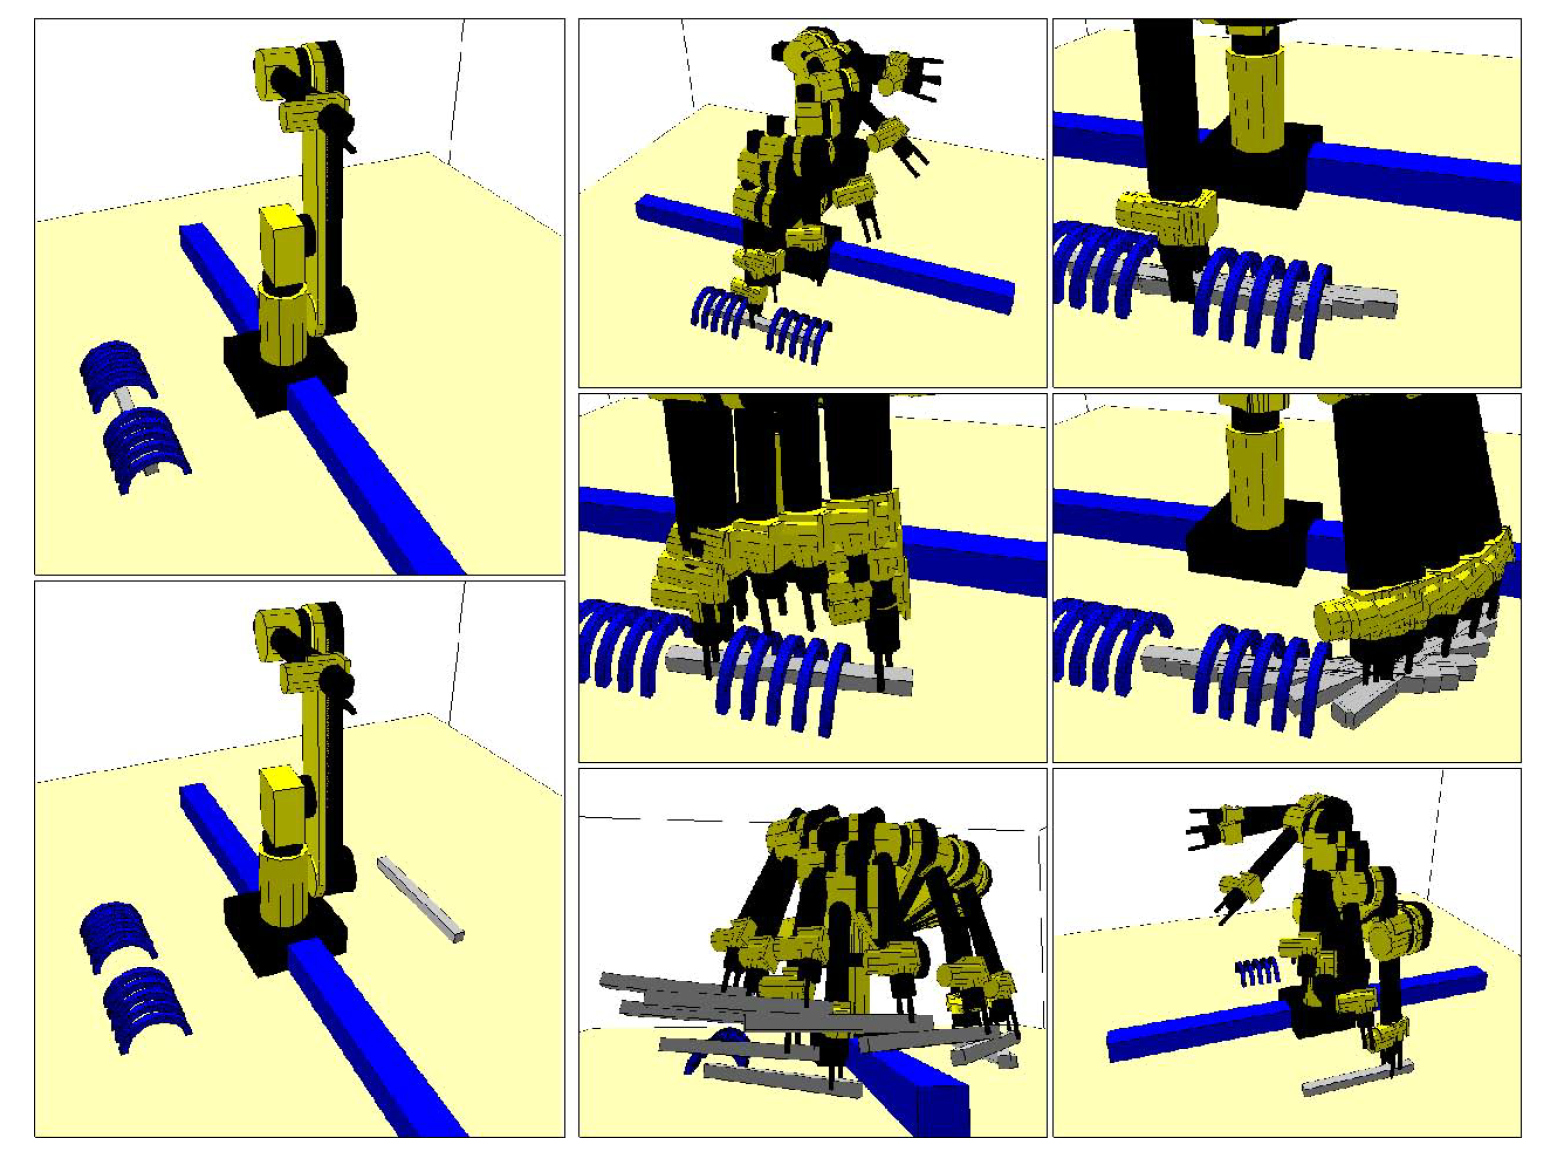
\includegraphics[width=0.75\textwidth]{images/hierarchical.png}
	\caption{Abb. 5.1 von \cite{cortes:03}: Wie kann das Objekt von seiner Ursprungsposition (oben, links) zur finalen Position (unten, links) bewegt werden? Die Lösung (rechts) erfordert mehrere \textit{Verbschiebeoperationen}.}
	\label{cortes01}
\end{figure}

\section{Klassifizierung von Pfadplanungsalgorithmen} \label{Kapitel 3.2} 
Da die algorithmische Umsetzung der Pfadplanung stark von den Vorgaben des Einsatzgebiets abhängig ist, sind auch die Vorgehensweisen stark heterogen.
Es wird Planen in einem diskreten und in einem kontinuierlichen \textit{Zustandsraum}\index{Zustandsraum} unterschieden. Planen in einem kontinuierlichen Zustandsraum wird Bewegungsplanung genannt, dabei wird Planen mit allen Umgebungsinformationen, Planen mit Unsicherheit und Planen mit Bewegungseinschränkungen unterschieden\cite[~S. 24-26]{Lav06}.
Im Kapitel \ref{Kapitel4} werden Anwendungen behandelt, die sich den Gebieten zuordnen lassen. 
 Die diskrete Pfadplanung dient als Grundlage auch für weitere Algorithmen, da letztendlich auch viele Probleme im kontinuierlichen Zustandsraum mit diskreten Methoden gelöst werden\cite[~S. 25]{Lav06}. 

\section{Diskrete Pfadplanung} \label{Kapitel 4.3} 
Der Zustandsraum ist bei der diskreten Pfadplanung entweder endlich, oder \textit{abzählbar unendlich}\index{abzählbar unendlich}.
Damit müssen keine geometrischen Modelle, oder \textit{Bewegungseinschränkungen}\index{Bewegungseinschränkungen},  im Entwurf des Algorithmus beachtet werden.
% Der Planer weis über alles bescheit, die struktur ist regelmaeßig
Je nach Anforderung werden die drei Teilgebiete \textit{feasible planning}\index{feasible planning}, \textit{optimales Planen}\index{optimales planen} und \textit{Logik basierte} Repräsentation unterschieden\cite[~S. 27]{Lav06}.
% Die vorherrschenden Algorithmen in diesem Bereich, sind der Dijkstra-Algorithmus aus der Graphentheorie und der daraus abgeleitete A*-Algorithmus. Von diesem gibt es noch eine Reihe weiterer Abwandlungen, die alle eine Optimierung auf ein bestimmtes Einsatzgebiet zum Ziel haben. \\
%Wie man diese Optimierung durchführen kann wird im folgenden an verschiedenen Algorithmen erläutert. 
Optimales Planen unterscheidet sich nur insofern vom feasible planning, als das der gefundene Pfad in verschiedenen Kriterien wie Zeit, Distanz, oder auch der Anzahl an Drehungen eines Roboters optimiert werden kann\cite[~S. 43]{Lav06}.
Zwischen Zuständen kann, durch die Ausführung von Aktionen, gewechselt werden. Die verfügbaren Aktionen werden in einem Aktionsraum\footnote{Aktionsraum (engl. action space) } zusammengefasst, und ein Satz von Zielzuständen\footnote{Zielzustände (engl. goal states)} wird definiert. 
Da ein Zustandsgraph schnell sehr groß werden kann, wird dieser meist nicht komplett übergeben, sondern im Laufe des Planungsprozess aufgedeckt\cite[~S. 43]{Lav06}. 
Bei Formulierung \ref{lav03} ist der Vergleich mit einem DEA\index{deterministischer endlicher automat} interessant ist hier auch der Vergleich mit \cite[~S. 233]{Schmitz:19}.

\begin{figure}
\centering
\subsection*{Formulierung 4.3 (Discrete Feasible Planning)}
\begin{enumerate}
	\item Ein nichtleerer Zustandsraum $X$, der endlich viele oder zählbar unendlich viele Zustände beschreibt.  
	\item Für jeden Zustand $x \in X$ , ein endlicher Aktionsraum $U( \, x) \,$.
	\item Eine Zustandsübergangsfunktion $f$ welche einen Zustand  $f( \, x,u) \, \in X$ für jedes $x \in X$  und $u \in U( \, x) \,$ erzeugt. Die Zustandsübergangsgleichung ist von $f$ als $x' = f( \, x,u )\, $ abgeleitet.
	\item Ein Anfangszustand $ x_{I} \in X$.
	\item Ein Satz mit Zielzuständen $X_{G} \subset X$.
\end{enumerate}
\caption{In Anlehnung an Formulation 2.1 von \cite[~S. 29]{Lav06}}
\label{lav03}
\end{figure}

\subsection {Feasible Planning}
Beim FP werden Algorithmen in Form der in Abbildung \ref{lav04} gegebenen \textit{Forward Search} verwendet. Diese müssen systematisch vorgehen, dass heißt bei endlich vielen Zuständen, müssen alle besucht werden (Zeile 2). Besuchte Zustände müssen markiert werden, um wiederholtes absuchen zu verhindern (Zeile 9). Bei einem unendlichen Graphen reicht es aus, zu einer Lösung zu kommen, sollte diese vorhanden sein (Zeile 5).\cite[~S. 32]{Lav06}

\begin{figure}
	\centering
	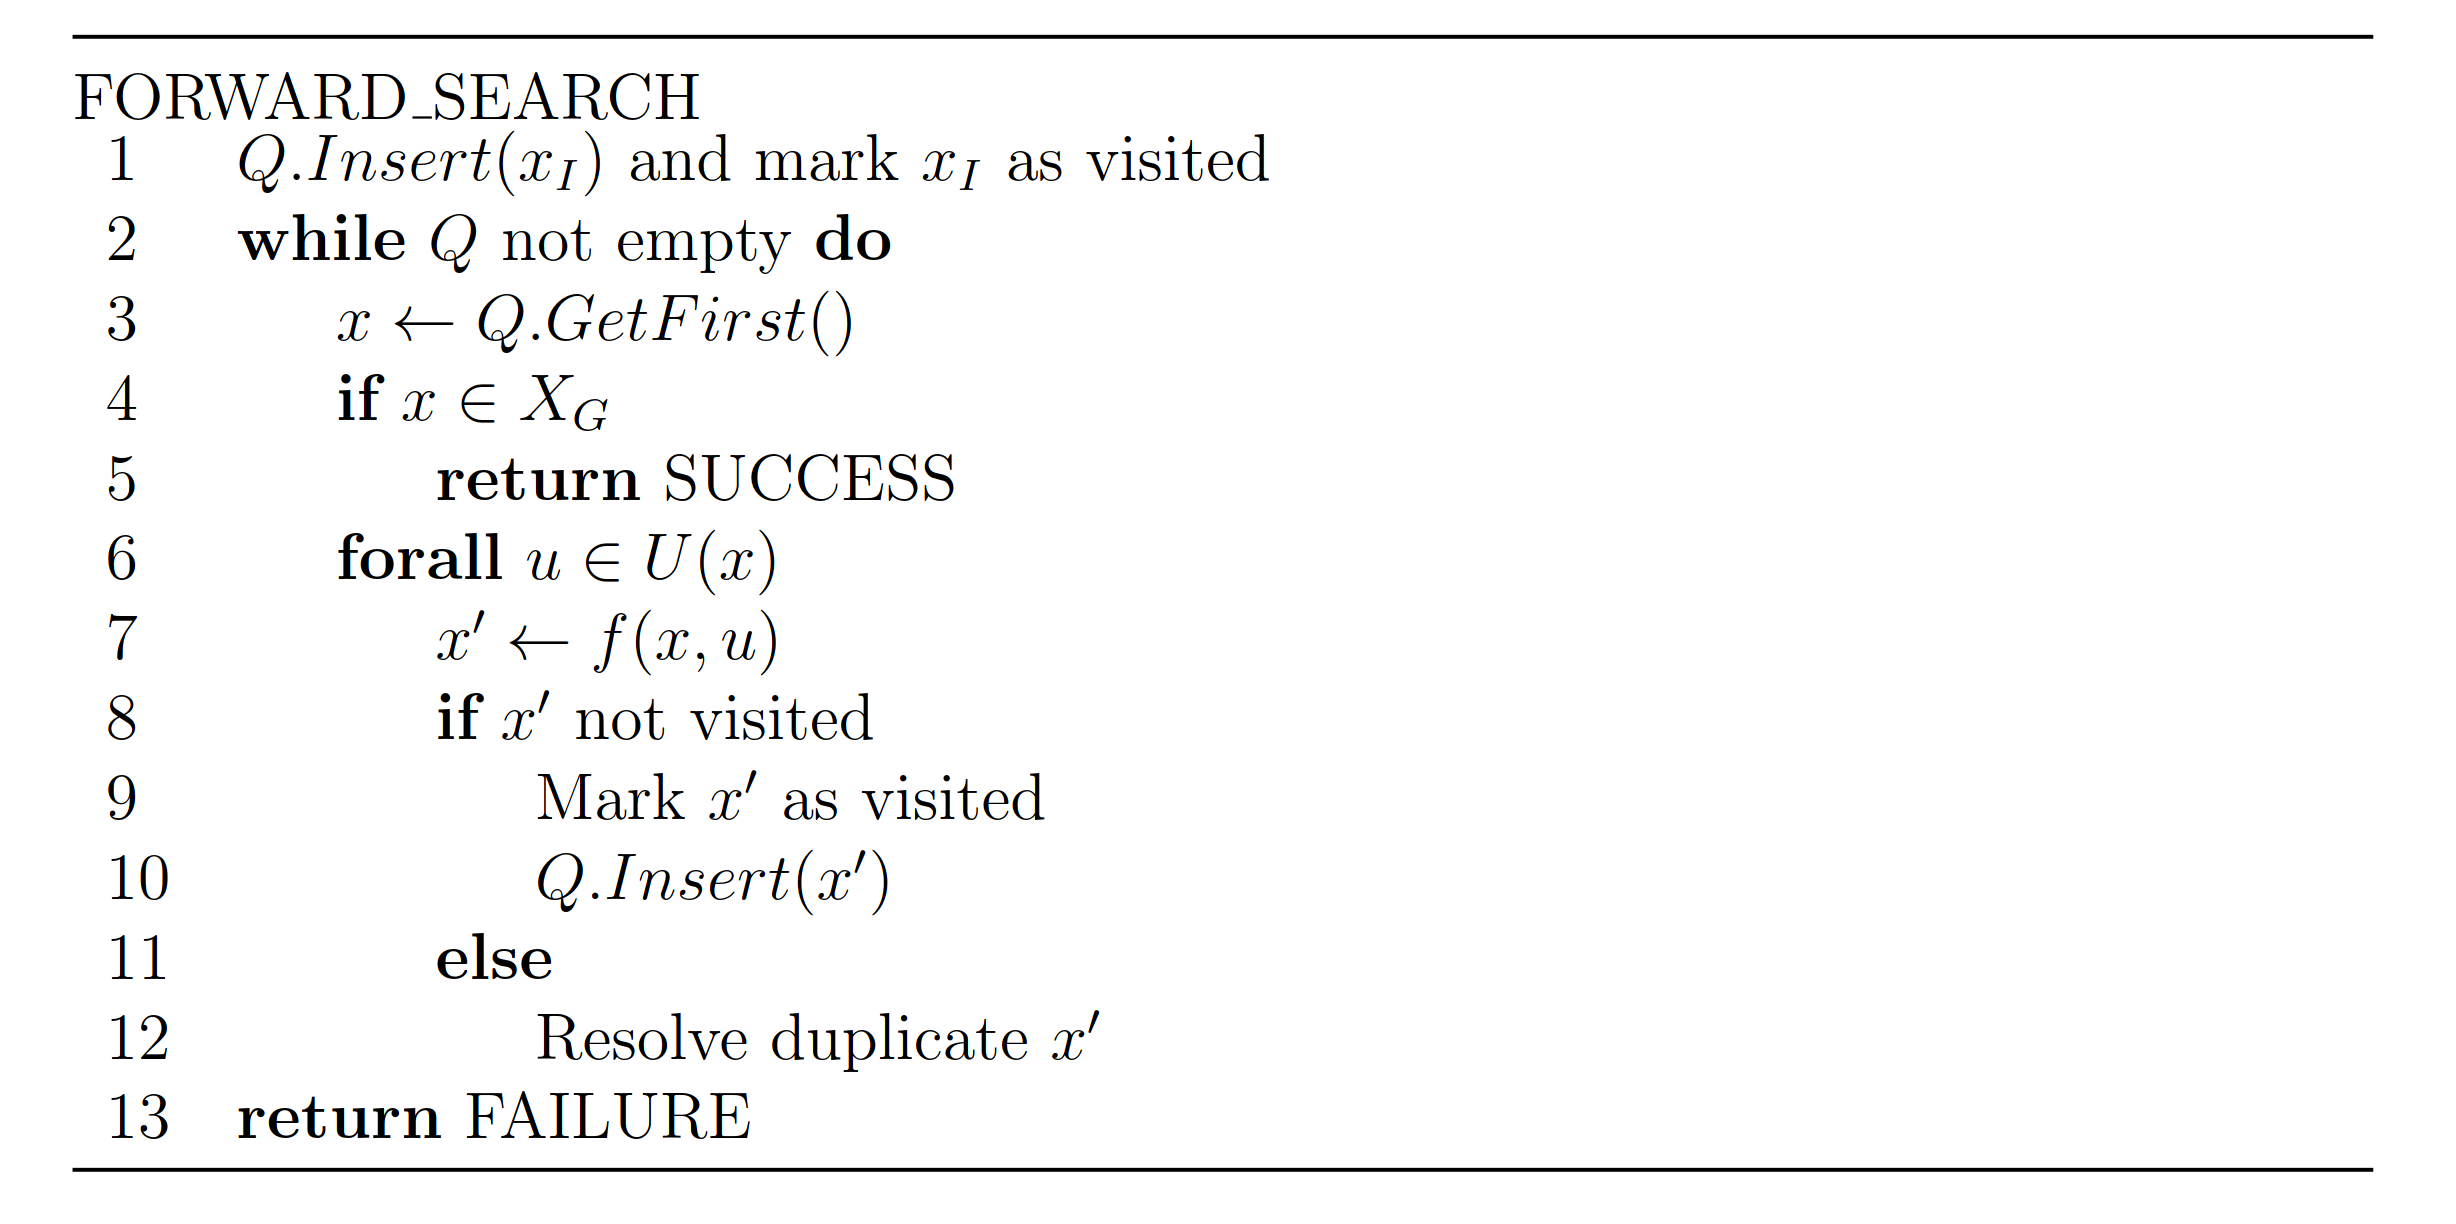
\includegraphics[width=0.9\textwidth]{images/img225.png}
	\caption{Abbildung 2.4 von \cite[~S. 33]{Lav06}:  Eine generelle Schablone für die vorwärts Suche.}
	\label{lav04}
\end{figure}
\noindent
Felder können drei Zustände einnehmen.
Ein \textit{unentdecktes} Feld wurde noch nicht besucht und ist daher auch noch nicht bekannt.
Ein \textit{totes} Feld kann nichts mehr mehr zur Suche beitragen, da alle angrenzenden Felder entdeckt wurden.
Ein \textit{lebendes} Feld hat noch mindestens ein Nachbarfeld das unentdeckt ist.
%
%Felder können drei Zustände einnehmen:
%\begin{enumerate}
%
%\item \textit{unentdeckt}: wurde noch nicht besucht und ist daher auch noch nicht bekannt.
%\item \textit{tot}: kann nichts mehr zur Suche beitragen, da alle angrenzenden Felder entdeckt wurden.
%\item \textit{lebend}: hat noch mindestens ein Nachbarfeld das unentdeckt ist. 
%\cite[~S. 33]{Lav06} 
%\end{enumerate} 
In der Warteschlange \footnote{Warteschlange (engl. priority queue)}, Abbildung \ref{lav04} (Zeile 1), werden die nächsten Felder gespeichert.Deren Sortierung hat einen großen Einfluss auf das Verhalten des Algorithmus wie an den Suchalgorithmen schnell deutlich wird. 
	\begin{itemize}
		\item Die einfachste Sortierung ist \textit{First-In First-Out}\index{First-In First-Out}, hier entsteht eine kreisförmig expandierende Suche. Dies wird im \textbf{Breath-first} Suchalgorithmus verwendet. Er ist systematisch und leicht zu kontrollieren, jedoch verschwendet er relativ viele Suchzyklen\cite[~S. 35]{Lav06}.
		\item Mit \textit{Last-In First-Out}\index{Last-In First-Out}, entsteht eine aggressive Expansion, in eine bestimmte Richtung. 
		Dies wäre ein erstrebenswertes Verhalten, die Richtung kann aber mit LI-FO nicht kontrolliert werden. Der \textbf{Depth-first} Algorithmus setzt das ein, er ist aber aber nur bei endlich vielen Knoten systematisch\cite[~S. 36]{Lav06}.
		\item Der \textbf{Dijkstra} Algorithmus vergleicht im Laufe der Suche Aktionen mit einander und erstellt so eine Warteschlange, die Knoten mit besseren Chancen bevorzugt. Im Normalfall sucht er solange, bis der optimale Pfad gefunden wurde. Das Vorgehen wurde zum ersten mal 1959 von E.W. Dijkstra im Artikel \cite{dijkstra:59} beschrieben.
		\item Der \textbf{A*-Suchalgorithmus}\footnote{A-Stern gesprochen} erweitert Dijkstra um eine Schätzfunktion, welche die geschätzten Kosten bis zum Ziel angibt.
		$$f( \, n ) \, = g ( \, n ) \, + h ( \, n ) \,$$
		So werden Knoten bevorzugt, welche die Suche möglichst schnell, näher zum Ziel bringen. Das daraus entstehende Verhalten zeichnet sich dadurch aus, dass der Algorithmus solange in Richtung des Ziels sucht, bis er auf ein Hindernis stößt. Erst dann versucht dieses zu umgehen. Es wird garantiert, dass immer der optimale Pfad gefunden wird.\cite[~S. 37]{Lav06}
	\end{itemize}
Um den gefundenen Weg zu rekonstruieren müssen die Vorgängerknoten jedes Knoten gespeichert werden. Dies würde man in Abbildung \ref{lav04} (Zeile 7) vornehmen. 


%Simon fährt fort
\section{Kontinuierliche Pfadplanung} \label{Kapitel 3.4}
%Wie unterscheidet sich Kontinuierliche Pfadplanung zu diskreter?
In der Pfadplanung im kontinuierlichen Zustandsraum\footnote{kontinuierlicher Zustandstraum (engl. continuous state space)}, auch Bewegungsplanung\footnote{Bewegungsplanung (engl. motion planning)} genannt, ist im Gegensatz zur diskreten Pfadplanung der Zustandsraum überabzählbar unendlich.  Der Zustandsraum ist zu groß, um explizit dargestellt zu werden. Dies liegt an der Anzahl oder der kombinatorischen Komplexität der Zustände \cite[~S. 17]{Lav06}.
Zur Veranschaulichung beschreibt Schwarz in \cite{Schw:83} das \textit{Piano Mover's Problem} als eine Aufgabe, bei der ein Körper einen kontinuierlichen Bewegungspfad durch einen Raum finden muss. Dabei gelten geometrische Einschränkungen, die es verbieten, mit den Hindernissen im Raum in Kontakt zu kommen.
 %evtl. S.157 Definition of basic motion planning + Formeln des PMPs (Formulation 4.1) einfügen.
Wie in \cite[~S. 79 f.]{Lav06} erläutert, gibt es zwei Motive, die bei der Pfadplanung im kontinuierlichen Zustandsraum immer wieder auftauchen. Zum einen implizite Repräsentationen des Zustandsraumes und zum anderen die Transformation von kontinuierlichen Modellen in diskrete.

Bei impliziten Repräsentationen geht es darum, dass es einen Unterschied gibt zwischen der Welt, in der sich die Modelle befinden und dem Raum, in dem das Planen stattfindet. Dieser Raum wird Konfigurationsraum genannt. Die Welt, in der sich die Modelle befinden, wird in geometrische 2D und 3D Modelle transformiert. Beispielsweise nehmen die Sensoren eines Roboters die Umgebung wahr und erstellen dann eine digitale Karte, mit der dann der Pfad geplant wird.

Da kontinuierliche Modelle in diskrete transformiert werden, werden viele Algorithmen, die diskrete Zustandsräume verwenden, in die Bewegungsplanung eingebettet. Diese Transformation kann auf zwei verschiedenen Wegen erreicht werden. Beim \textit{combinatorial motion planning} erstellt der Algorithmus eine diskrete Repräsentation, die das Ursprungsproblem \textit{genau} darstellt. Dies ermöglicht eine vollständige Pfadplanung, die garantiert eine Lösung findet, falls sie existiert. Beim \textit{sampling-based motion planning} tasten Algorithmen durch Kollisionserkennungsmethoden den Konfigurationsraum ab und führen mit Hilfe der entstandenen Ergebnisse diskrete Suchen durch.


%\subsection{Planung mit allen Umgebungsinformationen vorhanden}
%
%\subsection{Planung mit Unsicherheit}
%
%\subsection{Planung mit Bewegungseinschränkungen}

 
%%oder einer Grafik die ich noch schreiben muss. 
%\section{Bewegungsplanung}
%% Die Planung muss zusätzlich noch die Bewegung in der Umgebung in betracht ziehen. 
%\subsection{Sampling-Based Motion Planning}
%\subsection{Combinatorial Motion Planning}
%\section{Planen mit Unsicherheit}
%% Hier kommt noch unsicherheit in der Umgebung hinzu, also auch dynamische Systeme
%\subsection{Entscheidungstheorie}
%\subsection{Planen mit Unsicherheiten in der Sensorik}
%\section{Planen mit Differentilen Einschränkungen}
%% Hier müssen bewegungseinschränkungen die durch den Verwendeten Roboter einhergehen beachtet werden. 
%\subsection{Sampling-Based Planning under Differential Constraints}
